%%
%% This is file `main.tex'
%%
%% ------------------------------------------------------------------------
%% Copyright (C) 2022 Q.Tang
%% 
%% Licensed under the Apache License, Version 2.0 (the "License");
%% you may not use this file except in compliance with the License.
%% You may obtain a copy of the License at
%% 
%%     http://www.apache.org/licenses/LICENSE-2.0
%% 
%% Unless required by applicable law or agreed to in writing, software
%% distributed under the License is distributed on an "AS IS" BASIS,
%% WITHOUT WARRANTIES OR CONDITIONS OF ANY KIND, either express or implied.
%% See the License for the specific language governing permissions and
%% limitations under the License.
%% ------------------------------------------------------------------------

% !TeX encoding = UTF-8
\documentclass{bjtu-report}

\graphicspath{{figures/}}

\title{中文标题}
\laboratory{实验室}
%\laboratorylogo{./vi/lab.png} % 取消注释在封面添加实验室 logo
\author{\textup{XX}}
\advisor{XXX}
\scene{北京交通大学XX课程设计}
\repository{https://github.com/Tang1705/BJTU-Report}

\begin{document}

\makecover

\pagestyle{bjtufancy}
\setcounter{page}{1}
\pagenumbering{arabic}

\section{Introduction}
\newpage


\section{Scope and Contributions}
\newpage


\section{Method}
\begin{figure}[!htbp]
	\center
	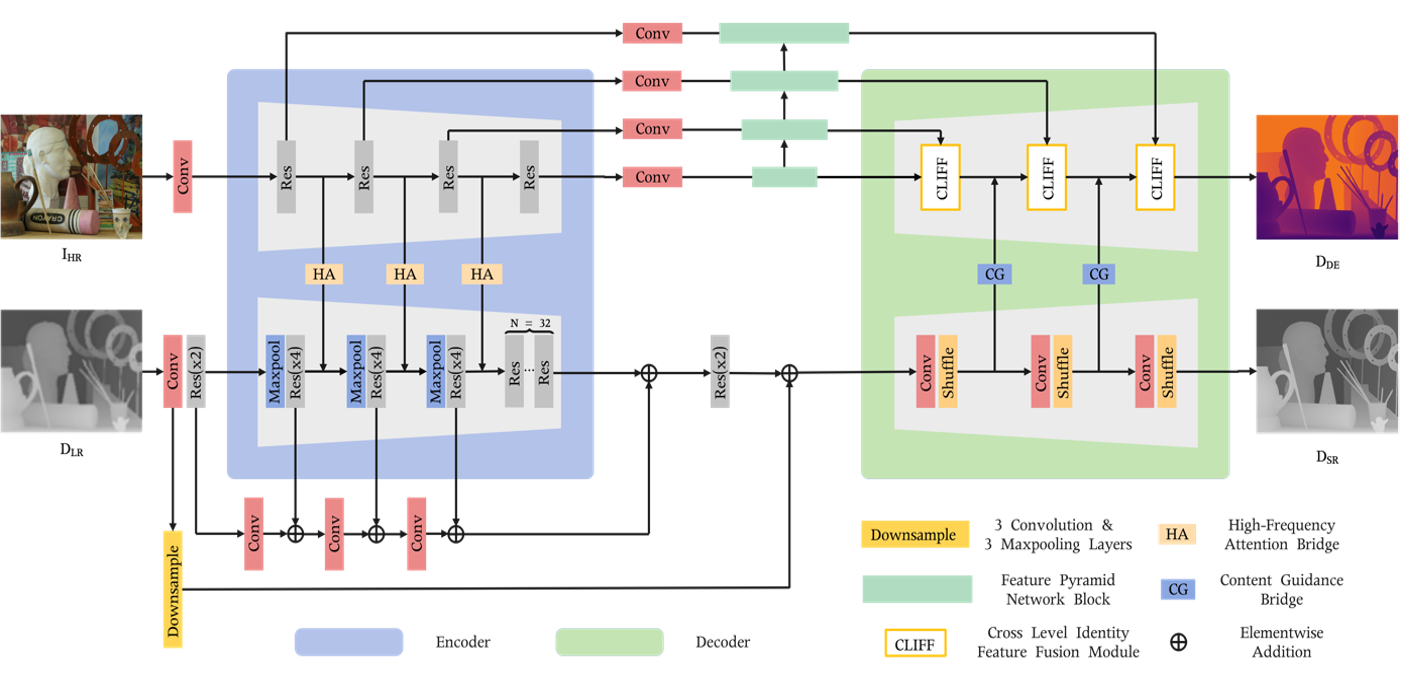
\includegraphics[scale=0.9]{mainnet.png}
	\caption{Overview of the proposed model}\label{fig:model}
\end{figure}

\subsection{Module1}

\subsection{Module2}
\newpage

\section{Experiments}



\end{document}

